
\documentclass{acm_proc_article-sp}


% Load basic packages
\usepackage{balance}  % to better equalize the last page
\usepackage{graphics} % for EPS, load graphicx instead
% \usepackage{times}    % comment if you want LaTeX's default font
\usepackage{url}      % llt: nicely formatted URLs
\usepackage{color}    % colors for comments
\usepackage{latexsym} % for checkboxes
\usepackage{tipa}  % for chi letter
\usepackage{subfigure} %subfigure
\usepackage{marvosym}   % Euro symbol
\usepackage{amsmath}  % math symbols
% \usepackage{caption}
\usepackage{subfigure}
\usepackage{url}

% llt: Define a global style for URLs, rather that the default one
\makeatletter
\def\url@leostyle{%
  \@ifundefined{selectfont}{\def\UrlFont{\sf}}{\def\UrlFont{\small\bf\ttfamily}}}
\makeatother
\urlstyle{leo}

% get rid of the copyright box.
\makeatletter
\let\@copyrightspace\relax
\makeatother


% To make various LaTeX processors do the right thing with page size.
\def\pprw{8.5in}
\def\pprh{11in}
\special{papersize=\pprw,\pprh}
\setlength{\paperwidth}{\pprw}
\setlength{\paperheight}{\pprh}
\setlength{\pdfpagewidth}{\pprw}
\setlength{\pdfpageheight}{\pprh}

% Make sure hyperref comes last of your loaded packages, 
% to give it a fighting chance of not being over-written, 
% since its job is to redefine many LaTeX commands.
\usepackage{hyperref}
% \usepackage[pdftex]{hyperref}
% \hypersetup{
% pdftitle={Interacting with Smart(er) Objects},
% pdfauthor={Marty Pye},
% bookmarksnumbered,
% pdfstartview={FitH},
% colorlinks,
% citecolor=black,
% filecolor=black,
% linkcolor=black,
% urlcolor=black,
% breaklinks=true,
% }

% create a shortcut to typeset table headings
\newcommand\tabhead[1]{\small\textbf{#1}}

% editing commands
\newcommand{\comment}[1]{}
\definecolor{Orange}{rgb}{1,0.5,0}
\newcommand{\todo}[1]{\textsf{\textbf{\textcolor{Orange}{[[#1]]}}}}
\newcommand{\bug}[1]{\textsf{\textcolor{Orange}{#1}}}


% check boxes
\newcommand*{\thecheckbox}{\hss$\Box$} 
\newenvironment*{checklist} 
{\list{}{% 
\renewcommand*{\makelabel}[1]{\thecheckbox}}} 
{\endlist} 

% inch symbol
\def\inch#1{#1$''$}

% subscript
\newcommand{\superscript}[1]{\ensuremath{^{\textrm{#1}}}}
\newcommand{\subscript}[1]{\ensuremath{_{\textrm{#1}}}}

% Images
% \myFigure	[ LABEL_PREFIX (optional) ]
%			{ FILENAME (without extension) }
%			{ CAPTION TEXT }
%			{ SHORT VERSION OF CAPTION TEXT }
\newcommand{\myFigure}[2]
{%
	\begin{figure}[!h]
		\centering
		\includegraphics[width= 0.95\columnwidth]{#1}
		\caption{#2}
		\label{#1}
	\end{figure}
}

% Footnote without symbol
\newcommand\blfootnote[1]{%
  \begingroup
  \renewcommand\thefootnote{}\footnote{#1}%
  \addtocounter{footnote}{-1}%
  \endgroup
}



% statistics report
\def\ANOVA#1#2#3#4{$F_{#1,#2} = #3, p = #4$}
\def\ANOVAS#1#2#3#4{$F_{#1,#2} = #3, p < #4$}
\def\tt#1#2#3{$t_{#1} = #2, p = #3$}
\def\tts#1#2#3{$t_{#1} = #2, p < #3$}
\def\Wilcox#1#2{$Z = #1, p #2$}
\def\GEE#1#2#3#4{Wald \textchi$^{2}_{#1,N=#2}=#3,\ p#4$}
\def\Mean#1{($M = #1$)}


% variable names
\def\PointingTime{\emph{ManipulationTime}}
\def\DriftCount{\emph{DriftCount}}
\def\Thickness{\emph{Thickness}}
\def\MovementDistance{\emph{MovementDistance}}
\def\SurfaceSupport{\emph{SurfaceSupport}}
\def\UserID{\emph{UserID}}
\def\SmallMovement{\emph{SmallMovement}}
\def\LargeMovement{\emph{LargeMovement}}
\def\HandOnSurface{\emph{HandOnSurface}}
\def\HandInMidair{\emph{HandInMidair}}
\def\Predepressing{\emph{Pre-depressing}}
\def\DragDepressing{\emph{DragDepressing}}
\def\ClickDepressing{\emph{ClickDepressing}}
\def\PreLeaving{\emph{Pre-leaving}}
\def\Leaving{\emph{Leaving}}

% End of preamble. Here it comes the document.
\begin{document}
\title{Interacting with Smart(er) Objects}
% \numberofauthors{1}
% \author{Marty Pye\\ RWTH Aachen University\\ marty.pye@rwth-aachen.de}
\maketitle
\begin{abstract}
The Internet of Things (IoT) is currently a rapidly growing field in computer science.
The amount of internet enabled devices and objects is growing vastly. 
The IoT concept is much broader than the familiar collection of internet enabled devices such as laptops, smartphones, tablets, etc.
It includes all sorts of everyday objects that previously did not contain electronic components, but are now sensing and communicating with each other and the internet (see Figure \ref{fig:iot}).

Careful consideration needs to be put into the interaction design concept of such objects, such that it does not interfere with the original purpose of the object, or at least merges well with that purpose.
Several challenges need to be met when embedding interaction in everyday objects.
These challenges include the invisibility dilemma, embedded vs.\ dedicated device interaction and implicit vs.\ explicit interaction, and are discussed in Section~\ref{sec:interaction}.
How these challenges have been tackled by previous researchers in their systems is then elaborated in Section~\ref{sec:caseStudies}. 
This thesis then concludes with a derived set of guidelines that developers in this area should take into account, so as not to succumb to the common pitfalls of designing interactive everyday objects.

The other component which needs consideration is the actual implementation of the connectivity and interactivity. Depending on the environment and context of the smart object, different protocols make more sense.
This thesis briefly presents the different technologies in Section~\ref{sec:techniques}.
On the basis of several research projects, the thesis then discusses, which communication protocols would make more sense if those projects were implemented in real-world scenarios.
\end{abstract}

\section{Introduction}
\label{sec:introduction}

The amount of internet enabled devices and objects is growing vastly, and the IoT concept is much broader than the familiar collection of internet enabled devices such as laptops, smartphones, tablets, etc.
It includes all sorts of everyday objects that previously did not contain electronic components, but are now sensing and communicating with each other and the internet (see Figure \ref{fig:iot}). Some real world examples are objects like buildings, household appliances, traffic members and even human bodies.
With the aid of sensors and microchips, they record various data like audio, temperature, movement, pressure, etc., and advanced algorithms and processing methods attempt to gain a deeper understanding of the environment and the user himself.

This paper first discusses the challenges of designing interactions with the internet of things in Section~\ref{sec:challenges}. 
It then elaborates on how these challenges have been tackled by previous researchers in their systems in Section~\ref{sec:caseStudies}, and then concludes with a derived set of guidelines that developers in this area should take into account, so as not to succumb to the common pitfalls of designing interactive everyday objects.
This paper also presents different technologies in Section~\ref{sec:techniques}, and discusses on the basis of several research projects, which communication protocols would make more sense if those projects were implemented in real-world scenarios.

The first section of this paper explores the IoT in more detail, and presents how the IoT can be separated into functional layers.

\section{The Internet of Things}
\label{sec:internetOfThings}
The internet of things (IoT) has been defined by the U.S.\ National Intelligence council as \emph{``the general idea of things, especially everyday objects, that are readable, recognizably, locatable, addressable, and controllable via the Internet - whether via RFID, wireless LAN, wide-area network, or other means \cite{disruptiveTechnologies}''}.
Everyday objects, which previously did not contain electronics are now being equipped with embedded sensors and microprocessors, and now communicate with each other and the internet. 
This allows for objects like buildings, roads, household appliances, human body parts and many more to be connected to the internet. 
The internet of things is undergoing a rapid growth. 
In 2008, the number of connected things exceeded the number of humans on this planet, and Cisco estimated that by 2020 we will have 50 billion things connected to the internet \cite{evans12}. 
Within this huge network of connected objects, a structure of functional layers is becoming apparent \cite{swan12}. 
As shown in Figure \ref{fig:functionalLayers}, the layers can be divided into the hardware sensor platforms layer, the software processing layer, the information visualization layer and the action taking layer. 
The following four sections briefly describe the responsibilities of each layer.
\begin{figure}[!t]
\centering
\includegraphics[width=0.9\columnwidth]{Images/IoT.pdf}
\caption{A variety of objects are joining the internet of things, and this paper discusses possibilities of interacting with it.}
\label{fig:iot}
\end{figure}

\begin{figure}[!t]
\centering
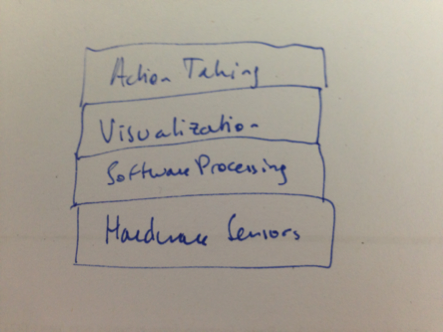
\includegraphics[width=0.9\columnwidth]{Images/functionalLayers.pdf}
\caption{Functional layers within the Internet of Things \cite{swan12}. The IoT is built upon low-cost sensors, which gather certain data. This data is then processed and possibly transferred to other devices, where it can be visualised and prompt the user to perform some action.}
\label{fig:functionalLayers}
\end{figure}

\subsection{Hardware Sensors}
\label{sec:hardwareSensors}
The whole IoT is built upon the increasing availability of low-cost sensors, which provide various kinds of functionality.
The common ones can sense movement, pressure, light, sound, electrical potential, temperature, moisture, location, heart rate, and many more.
It is common for one device to incorporate several sensing elements, which are usually driven by at least one microchip embedded in the sensing object.
This microchip is responsible for providing the sensors with power, gathering the sensor data, and then processing and/or forwarding it in some way.

\subsection{Software Processing} 
\label{sec:softwareProcessing}
Just gathering the data is usually not sufficient, it often needs to be processed and transmitted. 
The data processing can be done locally, on the device itself, or after the data has been transmitted. 
The advantage of processing the data immediately on the device is that the device does not need to uphold a network connection at all times. 
This is more demanding on the power source. 
However, depending on how computationally challenging the processing is, the chip might not have the resources to perform the processing. 
In that case, the data needs to be streamed to a more powerful, central unit. 
For the transmission, a variety of communication protocols can be used like Wi-Fi, Bluetooth, ZigBee, 3G, etc. 
A recent version of Bluetooth named Bluetooth low-energy allows mobile devices to send data with more battery efficiency. A brief overview over several communication protocols is provided in Section~\ref{sec:techniques}.

\subsection{Visualisation}
\label{sec:visualisation}
Once this data has been processed and transmitted, it often needs to be converted into some sort of human-readable form. The usual way of making the information accessible is through a graphical representation. 
Web interfaces and mobile applications have been created which display charts and statistics of the data, in an intuitively understandable manner. 
The data can be sorted on a time line, or according to events, depending on the use case.

\subsection{Action Taking}
\label{actionTaking}
The final step is the so-called action-taking layer, the layer which impels action-taking based on the acquired information. 
The information is presented in a context which makes it obvious to the user, what he should do as a result of having seen it.
This functionality is often the hardest to `get right'. 
The system needs to get across to the user what a good course of action would be, without being to obtrusive or demanding. 
The user should remain in control, or many people will be reluctant to use the system. The system should ideally be highly flexible and customisable, so that users can possibly set up actions about which they want the system to handle autonomously without their consent. It is possibly due to these issues that this layer is potentially the least explored so far.

\subsection{Contextualising}
Not all information gathered by sensors is aimed at being visualised and displayed to the user in some way. 
Very often, the sensors are used to give the object context awareness.
The sensors purpose is to gain some additional knowledge about the user or his environment, in order to influence the interaction on some higher level. 
The surrounding facts can enrich the interaction between human and device. 
Schmidt et al.\ \cite{schmidt99} derived a model in order to structure the feature space of context, as can be seen in Figure \ref{fig:context}.

\begin{figure}[!t]
	\centering
	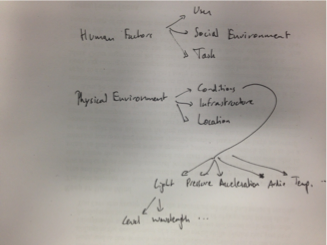
\includegraphics[width=\columnwidth]{Images/context.pdf}
	\caption{Feature space of context (Adapted from \cite{schmidt99}), which can be separated into context about the physical environment and human factors. Each of these can be divided up further, until low level factors can be measured by sensors.}
	\label{fig:context}
\end{figure}

At the top level, context related to human factors and context related to the physical environment can be distinguished. Each one of these categories can be separated into three further subcategories (see Figure \ref{fig:context}). Human factors can be sorted into information on:

\begin{itemize}
	\item The user: habits, emotional state, physiological condition, etc.
	\item The user's social environment: group, alone, social interaction, etc.
	\item The user's tasks: spontaneous activity, general goals, etc.
\end{itemize}

Context based on the physical environment can be sorted into information on:
\begin{itemize}
	\item Location: absolute or relative position, co-location with others, etc.
	\item Infrastructure: surrounding resources, communication network, etc.
	\item Physical conditions: noise, light, pressure, acceleration, etc.
\end{itemize}

Within each one of these subcategories, further features can be identified hierarchically. 
On the very bottom level, the values of those features can be measured by basic sensors, which can provide a basis for abstraction to higher level features. 
The fact that these values change over time provides additional context. 
The IoT trend is making more and more objects context sensitive by sensing one or many of the above features, examples of which can be found in Section~\ref{sec:caseStudies}.

If the object can be given certain levels of context sensitivity, the communication of the object with other objects and its environment can be improved.
The context can help the object rule out certain input, and therefore not have to transmit that data.
This is more energy efficient on the one hand, because the object has to send less data.
On the other hand, it's also preferable for the user, because unnecessary messages do not get passed to him.
Let's take a look at a concrete example.
Imagine a setting were the lights in a room are triggered by a motion sensor.
If there is no motion for a certain amount of time, the lights turn off.
This has the limitation, that if the user is quietly sitting at his desk, the motion sensors might not perceive his movement, and the lights then turn off.
This could be avoided by adding extra context awareness.
If the light controller could also keep track of the users location, it could decide to leave the lights when the user is in the room.
A system, which would enable such a set-up is NinjaBlocks, and is discussed in Section~\ref{sec:ninjaBlocks}.


Once smart objects have gathered some specific information, the user needs some means of interacting with the object.
This interaction often needs to occur prior to the data gathering, e.g.\ to set up the system, or subsequently, e.g.\ in order to retrieve and visualize the data. This can either occur directly on the object itself, through an application which augments the physical objects, or by speech.
Some different possibilities of interaction, together with their pros and cons are discussed in the following section.

\section{Interaction}
\label{sec:interaction}
In an IoT environment, objects need to be constantly modified or reprogrammed in order to fulfil the users' needs and requirements. 
Therefore, these objects need to allow some kind of interaction channel. 
Ideally, this interaction should be seamlessly and ubiquitously integrated into everyday artefacts, and it should allow input as well as output, depending on the application. 
Kranz et al. identified some key challenges of embedded interaction \cite{kranz10}, which are discussed in the following section.

\subsection{Challenges}
\label{sec:challenges}
Embedded interaction in the IoT provides many challenges to researchers. Some of the most prominent challenges are described in this section.

\subsubsection{Interaction devices vs.\ embedded interaction}
One approach to achieving interaction with everyday objects is using dedicated interaction devices which are connected to the object of interest when the interaction is required.
This has the advantage that the hardware necessary for the interaction can be removed when not needed (e.g. Smarter objects, see Section~\ref{sec:smarterObjects}), and can avoid accidental interaction. 
However, the interaction device may be unavailable at the given moment where it is required for interaction.

The alternative approach is embedding the interaction device into the everyday object, which means integrating interaction opportunities into existing artefacts (e.g. Pinstripe, see Section~\ref{sec:touchInputOnClothes}). 
The advantage of embedding the interaction is that the user can communicate with the object at any point in time, without having to worry about connecting an interaction device.
However, this can lead to accidental activation and input, and can be subject to a further challenge, known as the invisibility dilemma.

\subsubsection{Invisibility dilemma}
When augmenting an everyday object, it is important to preserve the original function, look and feel (e.g. Pinstripe, see Section~\ref{sec:touchInputOnClothes}.
Only then the user can continue utilising the object as before. Imagine a knife with several buttons on the handle. They would have to be arranged in order to assure that they do not get accidentally pressed when cutting with the knife.
However, if the interface is so hidden that it does not interfere with the objects original appearance, then the user might not be able to identify digital enhancement.
He might not recognise the object has added functionality.
Therefore, the interface needs to be very carefully designed, in order match the requirements of the application, without interfering with the original purpose or obstructing the everyday interaction with the respective object.

\subsubsection{Implicit vs. explicit interaction}
Explicit interaction means the user interacts with the object consciously, in order to achieve a certain goal.
He is fully aware of what he is currently doing.
Implicit interaction means the system is communicating in the background, while the user is performing some other action.
For example, the knife might be gathering information on the chopping speed while the user is cutting vegetables. Depending on the application and intended usage of the device, the choice of whether to use implicit or explicit interaction should be made carefully.
A knife where you have to count your chops/sec and manually enter the chopping speed at regular intervals would not be very user friendly.

\subsection{Technology}
\label{sec:techniques}
This section briefly introduces the technologies which are often used to establish the connectivity between devices. These are Bluetooth \cite{bluetoothPatent} or IEEE 802.11 (Wi-Fi).
\subsubsection{Bluetooth}
The main features of Bluetooth are ubiquity, low power consumption, and low cost \cite{btbasics}.
A wide range of devices can connect and communicate with each other when in proximity to one another.
The devices communicate through a short-range, ad-hoc network, also known as a piconet.
These piconets are established automatically as soon as the devices enter radio proximity, and they can connect whenever convenient.
Therefore, Bluetooth technology is suitable for objects that are going to be in close proximity to one another. 

\subsubsection{Wi-Fi}
Another communication protocol often used is IEEE 802.11 (Wi-Fi).
Wi-Fi enabled devices are able to connect to a network resource through a wireless access point, which has a limited range.
If the access point is so configured, they are able to connect to the internet.
Therefore, Wi-Fi is a suitable protocol when the smart objects need to communicate with any kind of internet services.

\subsection{Interaction Techniques}
This section describes some typical interaction techniques which can be used in the internet of things. Interactivity can be achieved by either making the objects smarter, or making the environment smarter.

Embedding the technology inside the objects has the disadvantage that they need to have their own power source.
This makes them sensitive to water and delicate if the electronics are not well enough protected.
Kranz et al. created some smart kitchen utilities as prototypes in order to demonstrate characteristic interaction methods \cite{kranz10}. 
One of these was a pressure sensitive cutting board, which senses the weight of the food prepared on it. 
Embedding electronics like this in various kitchen utilities may be challenging, as bread boards and many tools used in the kitchen need to be washed. 
Therefore, the electronics need to be waterproof, which again tends to make the components less accessible for things like changing the battery.

Another alternative to make objects smart is to augment the environment instead of the object itself. 
This has the advantage that the objects themselves do not require any embedded electronics, a power source, nor do they need to be connected to the internet. 
Only the system which monitors the objects needs to have the computational functionality. 
The disadvantage of this technique is that it reduces the variety of sensing possibilities, the most common of which include visual sensing technologies. 
They are comparatively cheap and easy to set up. 
Examples for this are World Kit \cite{xiao13}, Instant User Interfaces \cite{corsten13}, iCon \cite{cheng10} and Opportunistic Controls \cite{henderson08}. 
These systems allow quick and flexible augmentation of everyday objects, but are very susceptive to problems like occlusion and lack of precision.
Other approaches can include audio sensing technologies, like StickEar \cite{yeo13}. Let's take a look at some of these exemplary systems which use augmentation of the environment.

\subsubsection{WorldKit}
\label{sec:worldKit}
The aim of this system is to allow touch-based interactive surfaces to be created on basically any surface \cite{xiao13}. 
This surface does not have to be modified in any way, and does not need to be calibrated for interaction in advance. 
From a user perspective, it is so easy to create interfaces on surfaces, that they could be repainted every time they are needed. 
Basically the user paints the user interface by stroking backwards and forwards over the surface. 
This movement is captured by a depth camera, and the area is highlighted by projection of a beamer. 
UI elements like sliders or buttons can be placed in this area, and saved by the application. 
For example, a typical living room has several sitting locations. 
The user sitting down about to watch television could create the controls on a table in front of him, or on the armrest of the couch he is sitting on (see Figure \ref{fig:worldkit}).
\begin{figure}[!t]
	\centering
	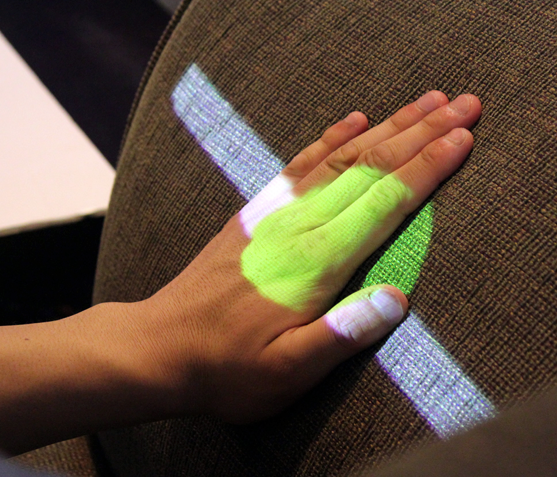
\includegraphics[width=0.9\columnwidth]{Images/worldkit}
	\caption{A user interface element spontaneously created on an everyday object (couch) \cite{xiao13}.}
	\label{fig:worldkit}
\end{figure}

This system does not quite fit inside the IoT, as the objects are not really made smart in any way. 
All this system does is create interfaces known to computers on top of everyday objects. 
The only sensing done by the system is whether the object is touched or not. 
It is not context sensitive, so accidental touching of the control interfaces could lead to unintended input. 
This demonstrates how visual sensing technologies, although practical from a technical perspective, come with some serious limitations. 
They need to be taken carefully into account, in order to create a system, which is actually useful and usable for the user.

Although the interaction is not strictly embedded in the object, rather temporarily created as an overlay, the challenges of embedding interaction still largely apply.
The authors chose to use explicit interaction, which in this scenario was a sensible choice.
The system implicitly guessing where a suitable place for a specific control would be is probably a little far fetched. 
False positives would lead to annoyance and confusion on the user's side.
They handled the invisibility dilemma by projecting the interface on the everyday objects.
Expert users of this system might be able to make use of the interaction without any visual feedback. However, projecting a volume control on an armrest for example could lead to accidental activation in the long run, by users placing their arms on the armrest, as was originally intended.
The authors handled this problem by creating a stroking gesture, which makes the creation and removal of interfaces on the surface very easy.
This gesture is suitable, as it does not often occur during normal use, except possibly during cleaning tasks.

Xiao et al.\ do not discuss how to implement the communication between the various objects that can be controlled through WorldKit interfaces.
Obviously the Kinect is connected to a computer which processes the image, but how should the computer then control whatever the user is trying to manipulate (e.g.\ TV, lights, radio,...)?
NinjaBlocks is a user-friendly approach to connecting these everyday objects.

\subsubsection{NinjaBlocks}
\label{sec:ninjaBlocks}
In order for applications like WorldKit to work, controllable devices need to be connected to the network.
Modern TVs are starting to have network connections, but a lot of simpler devices like radios, lights, blinds, windows, etc. do not have this connectivity yet.
Solutions for easily connecting these objects and making them controllable exist, one of them being NinjaBlocks\footnote{\url{http://ninjablocks.com/}}.
This is a platform which consists of small cloud-enabled computation units, that can sense their environment by using different sensors. 
The central unit of this platform is the so-called spheramid.
All the sensors stream their data back to the spheramid, which supports Wi-Fi, Bluetooth, BLE and ZigBee.
This allows a multitude of devices to be supported by NinjaBlocks.
The spheramid can then control objects like lights, heaters, etc.\ through network enabled sockets. An overview of how the NinjaBlocks system works is depicted in Figure \ref{fig:NinjaBlocksOverview}.

\begin{figure}[!t]
	\centering
	\includegraphics[width=\columnwidth]{Images/NinjaBlocksOverview.pdf}
	\caption{Communication overview of the NinjaBlocks system. The spheramid receives data from various sensors, processes them based on rules defined by the user, and then controls devices through network enabled sockets.}
	\label{fig:NinjaBlocksOverview}
\end{figure}

From the user's side, the system is very easy to set up, and he does not have to possess any coding skills.
NinjaBlocks has an app, where you can create rules with a graphical user interface.
This helps users who do not have any existing programming knowledge to link their devices together.
The central spheramid can then control all the devices based on the rules that the user defined.

Not only could WorldKit use the NinjaBlocks technology to establish the connection between user defined controls and controlled device, it could also use a similar graphical UI to connect the everyday objects and their controls.
However, a graphical UI is not the only way to link the interaction with the functionality.
Other strategies exist, and three are discussed and evaluated by Corsten et al.\ in Instant User Interfaces \cite{corsten13}. 

\subsubsection{Instant User Interfaces}
\label{sec:InstantUserInterfaces}

The first part of Corsten's work consisted of different possibilities of programming everyday objects \cite{corsten13}.
They evaluated the user's preferences on the programming method.
The first programming method was a speech interface.
They used a Wizard-of-Oz style setup, so that the user would not be limited to a specific command or vocabulary.
They could then use sentences like ``when I push this button, please advance to the next slide'' to establish a mapping between the object and the target action.
For the second programming technique, the mapping was established by demonstration.
The user performed a gesture on the object to be programmed while controlling the target interface with an existing physical controller, e.g.\ clicking a pen and pressing the right arrow key, which linked the clicking of the pen with advancing the slide.
The third programming technique consisted of a dedicated graphical user interface (see Figure \ref{fig:iuigui}).
\begin{figure}[!t]
	\centering
	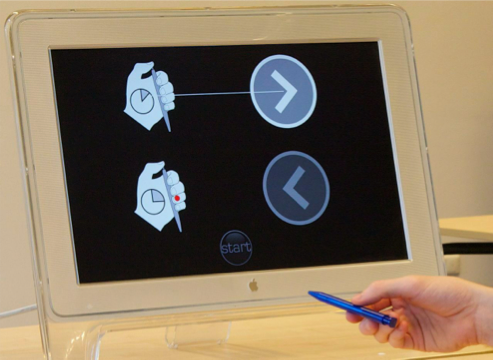
\includegraphics[width=0.9\columnwidth]{Images/IUIGui}
	\caption{GUI for Programming a pen as a remote. The left side lists the physical affordances of the object, while the right side lists the possible actions. \cite{corsten13}}
	\label{fig:iuigui}
\end{figure}

As a group the users did not have a clear preference towards one programming technique, but they did have distinct individual preferences.
It seems that providing several programming techniques would make sense, assuming they can all be reliably and unambiguously implemented.

The second part of Corsten's work consisted of creating an optical tracking system which allows marker less tracking of everyday objects.
The system could detect objects, their orientation in 3D space, as well as touches on that object. 
They propose using every day objects for instant user interfaces in order to improvise when a controller is missing but needed urgently, e.g.\ a pen to advance presentation slides instead of using the remote control.
Other than for improvisation, Instant UIs can be used for convenience, e.g.\ a stapler on a desk can be pushed to control a light, instead of having to get up and push the switch on the wall.
Instant UIs can also enhance usability, as selected functions which are crammed onto the remote can be outsourced to objects with better ergonomics and simple affordances.
Physical copies of existing controllers can be created when needed, e.g.\ an additional joystick for a multiplayer game when friends come over to visit.

Corsten et al.\ used an optical tracking system to sense the interaction, similar to Xiao et al.\ with WorldKit.
Again, the authors did not elaborate on how the system could control the lights, slides, etc. in the end.
If a system like this were deployed, a combination of this optical tracking and NinjaBlocks for example would seem to make sense.
The everyday objects like pens, mugs etc.\ could be made interactive without the need for adding electric components inside. After the user's action is processed by the camera, the NinjaBlocks system could then control the corresponding lamp, the TV volume, the presentation slides,... This would combine the advantages of optical tracking with the connectivity capabilities of NinjaBlocks.

The three programming techniques were chosen in this paper because they represent the diversity of existing programming techniques.
The speech interface is a virtual-to-virtual, the GUI a physical-to-virtual and the demonstration interface a physical-to-physical mapping technique.
Also, the speech interface is probably the most intuitive, the demonstration interface the most practical, and the GUI the most common programming method \cite{heun2013reality}, \cite{cheng10}, \cite{mayer13}.
The graphical user interface used by Corsten et al.\ was only very basic, as they were only looking to include that genre of techniques in their experiment. 
The following section investigates a more advanced system that explores a graphical method of interacting with everyday object more deeply.

\subsubsection{Smarter Objects}
\label{sec:smarterObjects}
Smarter Objects \cite{heun13smarter} is a system that enables rich, graphical interaction with everyday objects through a tablet or smartphone. 
As a user holds the tablet over a physical object, the augmented reality application recognises the object and offers a graphical user interface (see Figure \ref{fig:smarterObjectsGUI}), which can be used to modify the object's behaviour and interactions with other objects.
Once the object has been programmed, the GUI is not necessary anymore, and the object can be interacted with through its tangible interface (e.g.\ buttons, knobs).

Very often, the interaction with everyday objects can be separated into two different parts. 
The largest part of a user interaction is the daily operation. 
This interaction often only needs very little visual attention, as the object is fully understood and working as usual. 
The interaction is memorised by the user in muscle memory and skin feeling. 
The small part of possible user interaction is the customising or programming of these objects. 
For example, the user might want to preselect some specific radio stations as favourites. 
These steps require the most visual attention, but only represent a small percentage of the full interaction spectrum.
Heun et al.\ propose their AR application to provide a greater breadth of functionality and a more usable customisation technique during this interaction part, while maintaining the quick tactile interface for the larger, every day interaction part.

Other than providing a graphical interface for customisation and programming of everyday objects, Smarter Objects can couple different services and functions of these objects.
Smarter Objects can be easily linked by touching a tag on the GUI of one smart object and dragging it to the tag of a different smart object.
For example, the ``eject slider'' of a toaster could be linked to an alarm clock, so that the alarm rings when the toast pops out. 
Virtual smart objects can be placed in-between the interaction flow, so that for example, a Facebook message could make the light in the room blink several times.

\begin{figure}[!t]
	\centering
	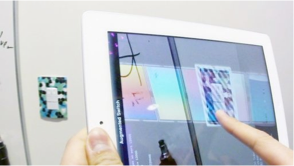
\includegraphics[width=0.9\columnwidth]{Images/smarterObjectsGUI}
	\caption{A graphical interface is displayed over a physical object in order to provide a richer control interface. \cite{heun13smarter}}
	\label{fig:smarterObjectsGUI}
\end{figure}

Smarter objects handles the challenges of making objects interactive quite well. 
An interaction device to set the objects functionality is only needed for the more complex setup purposes. 
After that, no or very little additional hardware is needed on the object itself.
Smarter objects combines explicit and implicit interaction.
First, the objects are explicitly programmed and coupled with the tablet application.
After that, the interaction between the smart objects happens implicitly. 
However, the invisibility dilemma still remains to some extent.
A user who did not set up the smart objects has no way of seeing that e.g.\ a light switch is connected with a toaster.
The system relies on the user remembering how his objects are interconnected, which scopes the applicability of this system down to private places, like homes, etc.

With regards to the structure of functional layers (Figure 1) in the IoT, Smarter Objects provides a kind of bridging capability between the bottom layer, and the top layer.
This avoids the technical overhead of having to traverse all the functional layers of the IoT.
However, this comes with the tradeoff, that the configuration is imposed upon the user. 
In order to demonstrate how a more advanced IoT system would work, imagine the following scenario: Bob wants his coffee machine to turn on when his alarm clock rings.
A potentially optimal system would not need Bob to do any configuration.
Sensors embedded in multiple everyday objects would be able to sense that every morning, when Bob wakes up, his first action is to turn on the coffee machine (Sensing Layer).
The intelligent system would then upon gathering this data learn (Processing Layer) that turning on the coffee machine when the alarm clock rings would be a suitable action (Action Layer).
The system could then either implement this rule itself, or suggest it to Bob in order to get his confirmation.
This would impose minimal cognitive load on Bob. 

\section{Case Studies}
\label{sec:caseStudies}
For the case that everyday objects should be made interactive by embedding technology inside them, they need to be augmented with input and output facilities.
As described in Section~\ref{sec:challenges}, the challenges of embedding interaction can be handled differently.
The following sections discuss some examples of embedding interaction in everyday objects.
Kranz et al. investigated several particular areas and their characteristic interaction methods \cite{kranz10}.

\subsection{Context-Aware Kitchen Utilities}
Kranz et al.\ created some augmented kitchen utilities, including a cutting board acting as a scale and a mouse interface, a sensor augmented knife and a sensor augmented table.
By sensing the weight of various food being chopped on the cutting board (Sensor Layer), the system can analyse whether more of an ingredient is required (Processing Layer).
The cutting board also acts a mouse interface, so that the user can control his computer without the need for clean hands.
This kind of interaction could easily be replaced with visual sensing technologies, whereas the weight sensing cannot.
However, the weight sensing could be enhanced through visual recognition, as the pressure sensors can't sense whether, for example, there is a knife lying on the board, adding to the weight.
If there were a camera however, which could detect the knife (similarly to \cite{corsten13}), and the system knew the weight of the knife, the board could deduct the weight of the knife and assess the portion size more accurately.
The smart knife can analyse the force and torque changes when the user cuts food, and infer the vegetable currently being cut.
Additionally, the sound of the vegetable being cut is also characteristic, and visual identification is also possible.
A combination of these techniques could provide reliable food detection.

The above scenario once again demonstrates the functional layer structure of the IoT.
From the basic sensing (e.g.\ weight, force, torque) the kitchen utilities can infer the context through processing (which food is being cut).
Although not suggested in this paper, the system could then e.g.\ visualise the percentage of the required vegetable that has been cut (Visualization) or suggest additional ingredients (Action-Taking) based on e.g.\ what is in the fridge, or the users nutritional data.

In this case, the smart kitchen utilities focus on implicit, unobtrusive interaction.
The sensors in the knife are hidden in the handle, the sensors on the board and the table hidden underneath.
Therefore, they do not interfere with the designated purpose and use of those objects, however, it is not necessarily apparent whether the objects are augmented or not (Invisibility dilemma).

\subsection{Capacitive Touch input on Clothes}
\label{sec:touchInputOnClothes}
Another domain of the IoT is smart clothing. 
Kranz et al. created an embedded interaction toolkit which lets designers quickly add interaction elements to clothes.
Their exemplary prototypes included phone bags, bicycle helmets, gloves and an apron with different layouts of touch controls.
They let different users try out the different prototypes in two user studies, first of which concentrated on gathering qualitative feedback and opinions about wearable computing in general, while the second evaluated the apron controls specifically.
As the authors did not elaborate any further on their studies, a more detailed approach is discussed in the following part.

Karrer et al.\ created Pinstripe \cite{karrer11}, which is a textile user interface element for eyes-free interaction on smart clothing, which uses pinching and rolling of the cloth between fingers as input (Figure 5).
\begin{figure}[!t]
	\centering
	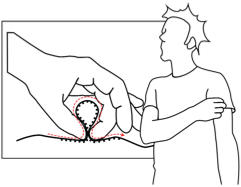
\includegraphics[width=0.9\columnwidth]{Images/pinstripe.pdf}
	\caption{The pinstripe control element functions by pinching and rolling a fold of cloth between your fingers. This can be used to control a linear value. \cite{karrer11}}
	\label{fig:pinstripe}
\end{figure}
The interface elements consist of parallel lines of conductive thread sewn straight into the fabric, so that they can be invisible.
There are several challenges when designing smart textiles.
\begin{itemize}
	\item \emph{Wearability} demands that the electronic components do not influence the main purpose of the clothing e.g. comfort, insulation, fabric breathability. 
	\item \emph{Fashion compatibility} demands for the electronic components not to interfere with the visual look of the clothing. 
	\item \emph{Durability} demands that the smart textiles be resistant against the strains of regular use.
	\item \emph{Interaction} which controls the fabric itself also needs careful consideration.
	The actions should not be triggered involuntarily, and as people are often moving, they should be able to interact eyes-free and single handedly.
\end{itemize} 

In their study, Karrer et al.\ used 16 potentially suitable areas for the Pinstripe element on the human body. The areas are depicted in Figure \ref{fig:areasBody} 
Participants in three different conditions (standing, walking, sitting) were asked to grade how convenient the different places were.
The most preferred area was the upper arm of the non-dominant arm (27,8\%), followed by the dominant hip (13,3\%) and the sternum (10\%).
Of the people who wore long sleeves, 43\% preferred the forearm of the non dominant hand, where as 25\% preferred the upper arm.

\begin{figure}[!t]
	\centering
	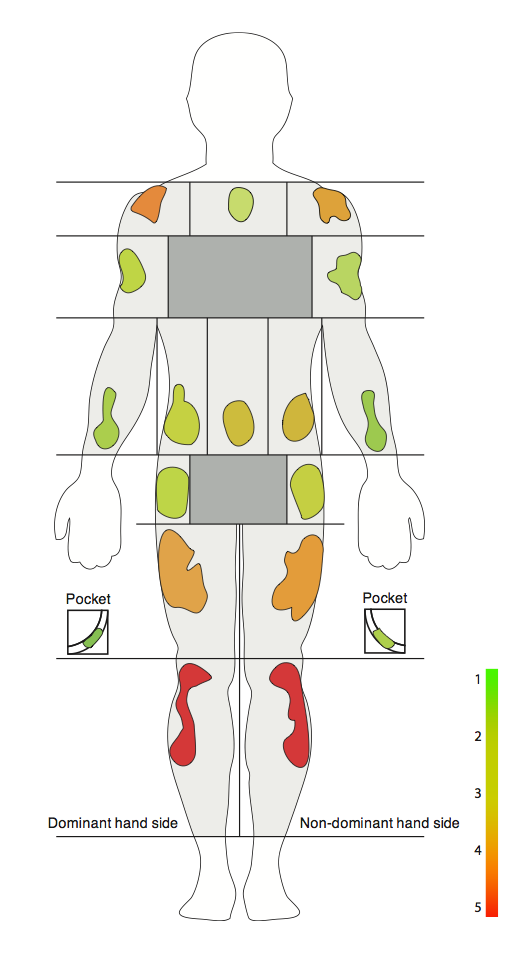
\includegraphics[width=0.9\columnwidth]{Images/areasBody.pdf}
	\caption{Karrer et al.\ selected 16 areas from the front of the human body where textile UI elements could be placed. Certain areas were excluded deliberately. The blobs outline the parts of each area where study participants grabbed a fold. Each blob is coloured-coded with the average grade given to that area. \cite{karrer11}}
	\label{fig:areasBody}
\end{figure}

Overall, the best suited area therefore may be the upper arms.
People are not always wearing long sleeved garments, and the sternum, although achieving good results in the walking condition (probably due to the reduced movement in comparison to arms and legs), was flagged as a socially unacceptable area for interaction by two participants.
Also, clothing with low necklines  would not allow interaction in that area.

Pinstripe is another good example of a system which tackles the challenges of embedding interaction in everyday objects well.
Unlike the kitchen utilities, Pinstripe focusses on explicit interaction, while attempting to hide the interface elements as much as possible.
While this makes the functionality less apparent, it makes sense in this case, as the elements are designed to be usable eyes-free.
Karrer et al.\ did not suggest any techniques for connecting the Pinstripe controls with the devices they are supposed to control.
However it seems, that a programming technique as used in Smarter Objects \cite{heun13smarter} would make sense here, as once the user has established what to use the control for, he is unlikely to change it very frequently.
A programming method by demonstration \cite{corsten13} as suggested by Corsten et al. also seems like a good candidate.

Finally, the Pinstripe interaction has to be connected to some application, in order to serve as an input device.
One can imagine many applications of an interaction technique like Pinstripe, and the authors tested three test applications.
They used Pinstripe to control three applications: The volume of a music player, a graphical menu and play list controls. 
As this was a prototype, the applications ran on a notebook which was in the user's backpack.
However, a version of the control circuit under development already allowed direct control of an iPod music player.
When first introduced to the Pinstripe clothing, the users expected functionality similar to a trackpad or an interactive surface. Once they had been shown by the experimenter, they were all successfully able to use Pinstripe.

Pinstripe as an example, one could imagine the connectivity to be implemented with Bluetooth.
The Pinstripe garment could register as a Human Interface Device with a Computer.
It could then act as any other peripheral device, like a keyboard, mouse, joystick, etc. 
No additional software would have to be installed on the computer. 
However, the garment would always have to be within reach of the computer.
Another alternative would be to implement 3G or Wi-Fi functionality for Pinstripe.
Roaming would then become easier for that garment, but there would have to be a server application running on the Computer/Tablet/Phone, which received the data from the garment. 
That application could then e.g. send control commands to the device which is intended to be manipulated.

\section{Conclusion and Guidelines}
\label{sec:conclusion}
Based on the experiences of Kranz et al.\ in the field of embedding interactions in everyday devices \cite{kranz10}, the following paragraph lists some important design guidelines.
Unless referenced otherwise, all guidelines were proposed by Kranz et al.
They believe that many problems and issues in the initial phase of projects in this field could potentially be avoided by following these guidelines.
\begin{itemize}
	\item \emph{Information when and where it's useful.} Information should be provided in order to let the user make more informed choices. Information should be shown in particularly at points where the user has to make a decision.
	\item \emph{Provide information without explicit interaction.} In some cases it might be useful for the user to be given information without asking for it, by exploiting a screen saver, for example.
	\item \emph{Overprovision}. Try and give the user multiple methods for achieving the same task, or viewing the same output. The IoT should provide many opportunities and remove limits and constraints between objects and devices.
	\item \emph{Specialized components}. Some times, a specialized device or interaction technique for a specific task is advantageous. This can be more efficient than an all-in-one device such as a smart phone \cite{corsten13,kranz10}.
	\item \emph{Invisibility dilemma.} The trade-off between clearly visible controls and those seamlessly integrated into an existing product design need do be considered carefully. From the examples explored in this paper, a general rule of thumb seems to be: If the interaction is explicit, make the controls clear and visible. If the interaction is implicit, try and integrate the technology as much as possible.
	\item \emph{Accidental use}. Accidental activation should be avoided. If users are afraid of initiating actions involuntarily, they might desist from using the device entirely.
	\item \emph{Short- and long-term life cycle.} The devices need to run for a sufficient amount of time before they need recharging or replacing. Always try and maximise the life-span of the device, and make the access to the technological components (e.g.\ batteries) easy and convenient.
	\item \emph{Rapid Prototyping}. In order to effectively explore the design space, try and employ cheap and fast prototyping tools to create early prototypes.
	\item \emph{Modelling support}. Provide support for formal models (e.g.\ Keystroke Level model, GOMS, etc.). This can save a lot of time and effort and help predict metrics such as task-completion times.
\end{itemize}

Embedding the interaction in the object is the first step, which already needs a lot of consideration.
The second step is deciding which communication protocol to use between the objects and the central processing unit.
This should be chosen with regard to how the objects will be used. If the objects will be roaming a lot, it makes more sense to use cellular network.
If the objects will probably only move locally, it makes more sense to use Wi-Fi or Bluetooth. In the future, we need intelligent frameworks which allow the connection to be set up as autonomously as possible, with as little configuration from the user side as possible.
The same applies to connecting the functionality of the smart objects.
The user should not have to be a programmer to create rules.
Graphical user interfaces, speech and demonstration can be used in order to provide an intuitive and natural programming technique.


\bibliographystyle{abbrv}
\bibliography{i4Seminar}

\balancecolumns
\end{document}
